\section{Varying Nodes: 50 and 700 cases}
At the edges of the node numbers chosen for our configurations we have 50 and 700. We now want to analyze the performance indixes for 50 and then for 700 nodes, to discover any similarities and/or differences with the case at 200.

\subsection{Coverage percentage}
\begin{figure}[H]
\minipage{0.50\linewidth}
  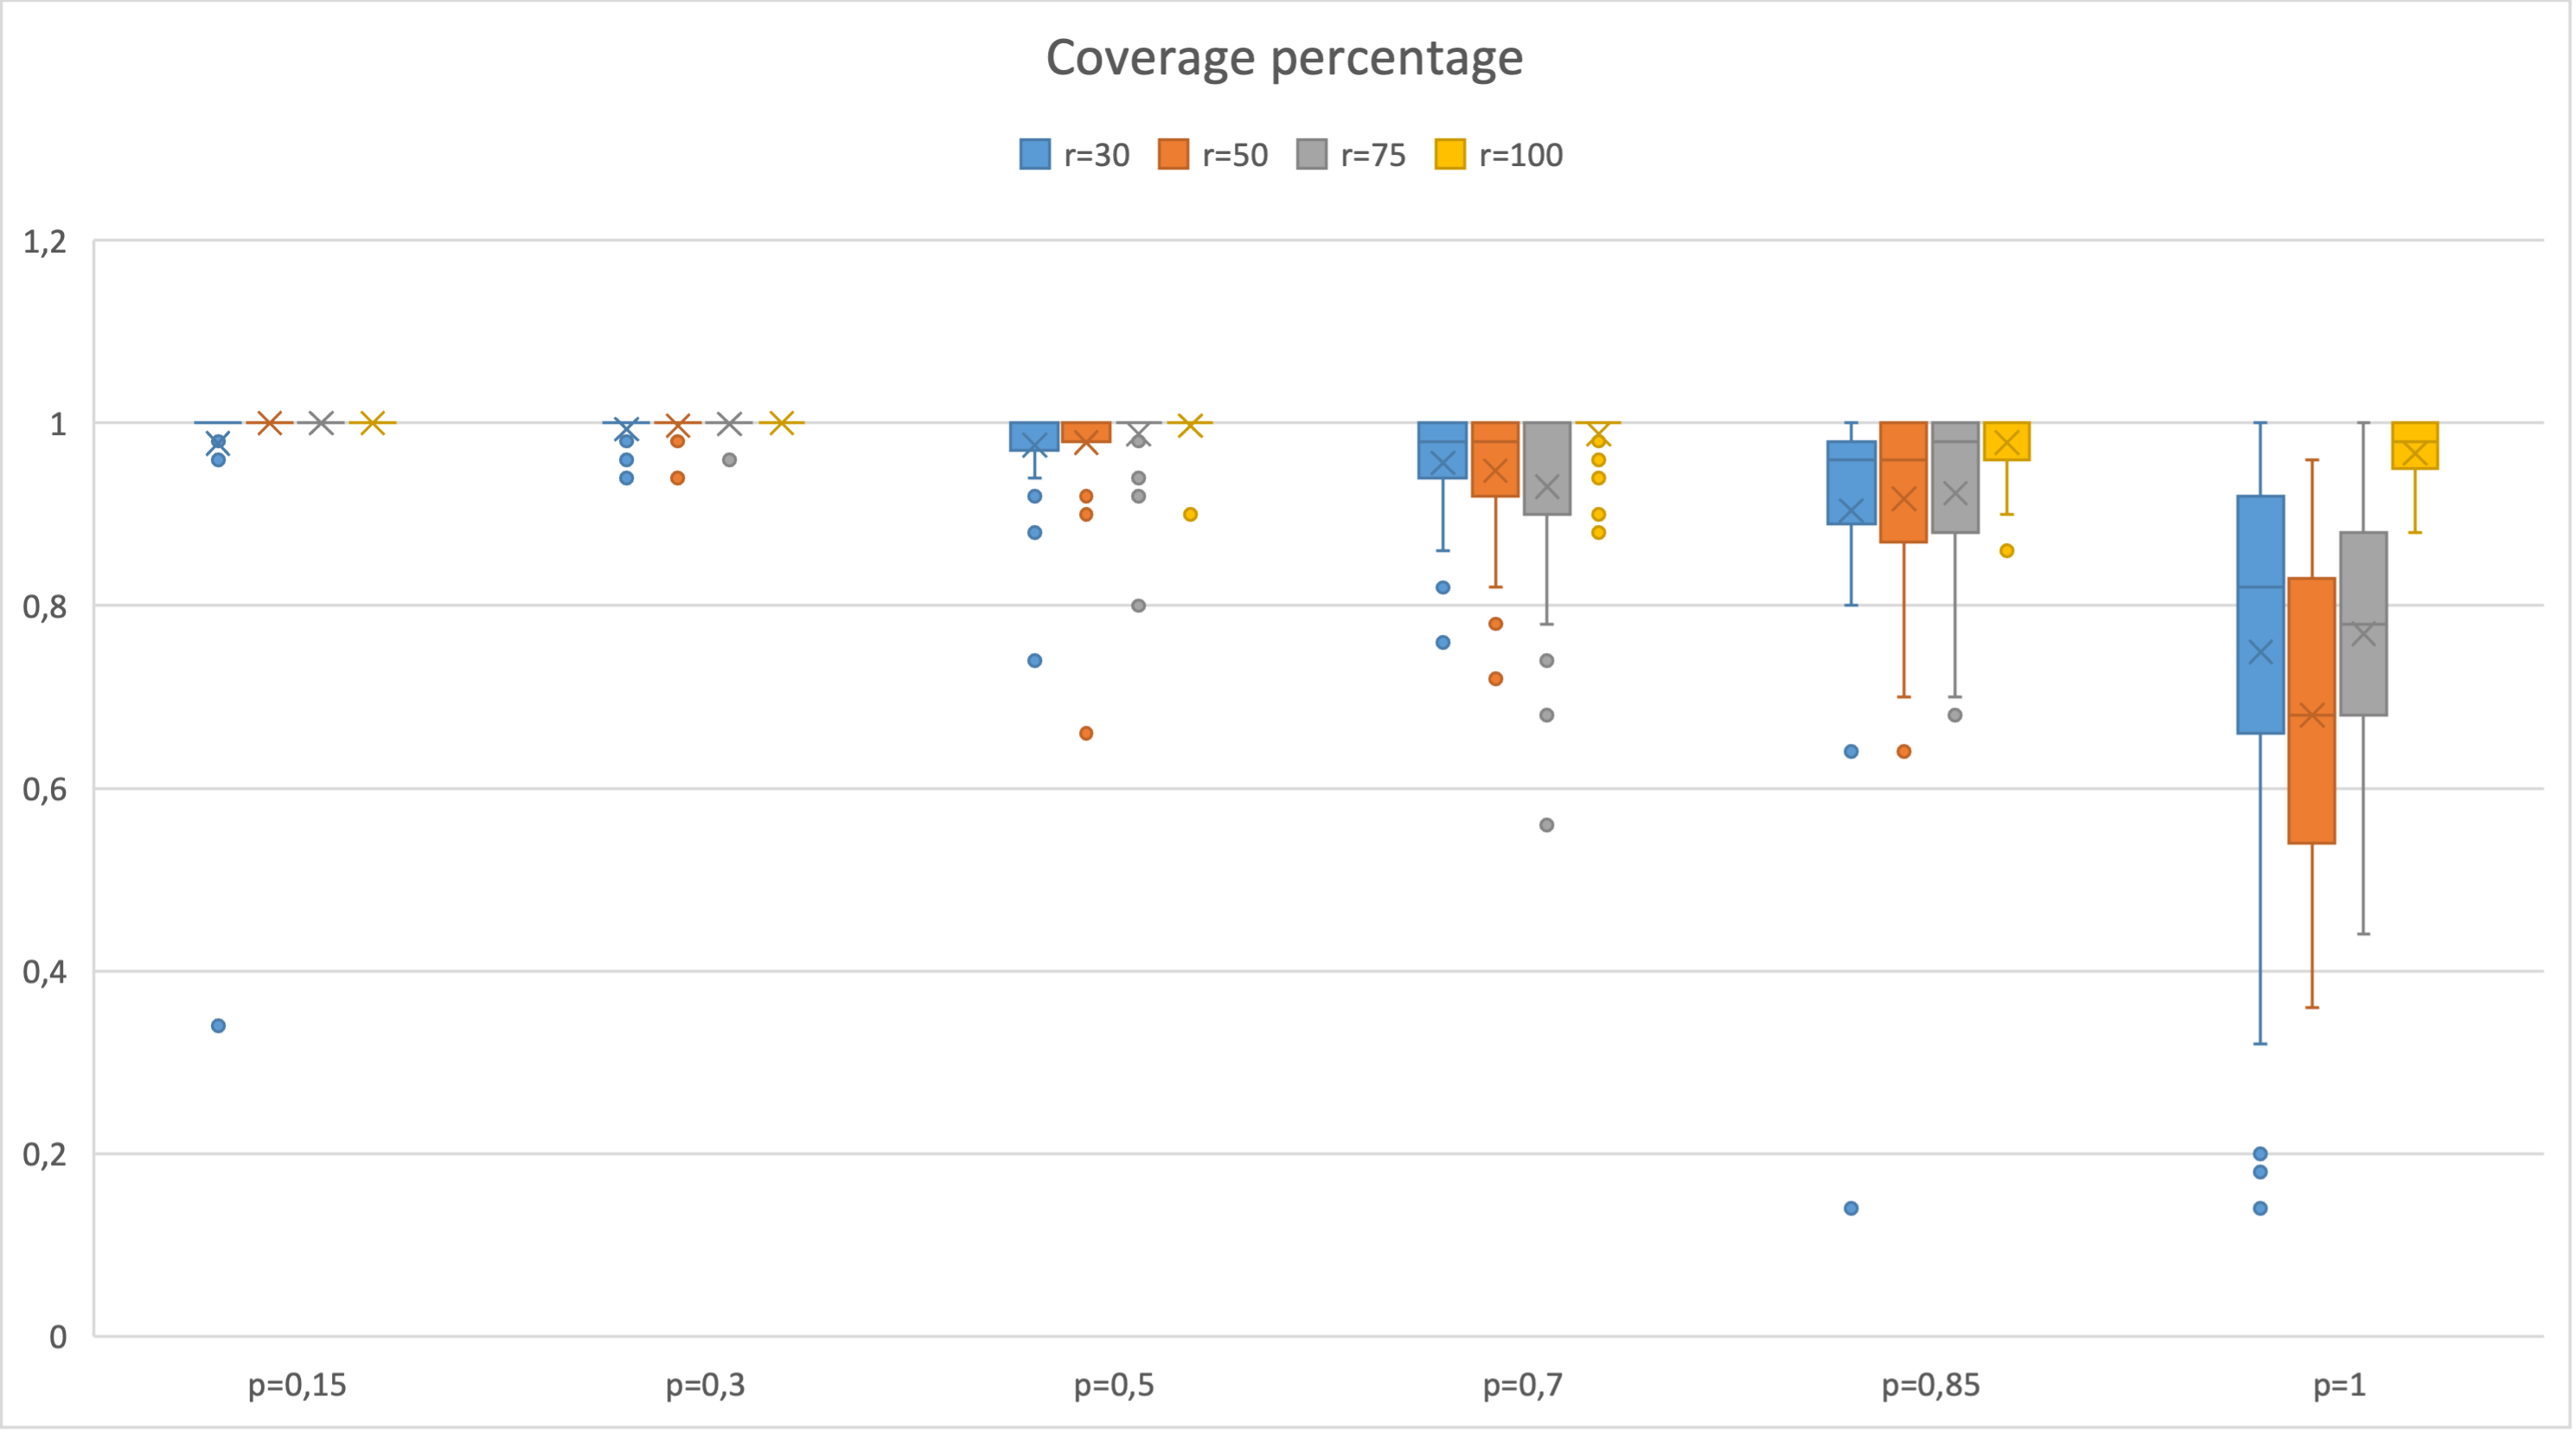
\includegraphics[width=\linewidth]{./images/Rate50Boxplot.png}
  \caption{50 Nodes}\label{fig:awesome_image1}
\endminipage\hfill
\minipage{0.50\linewidth}
  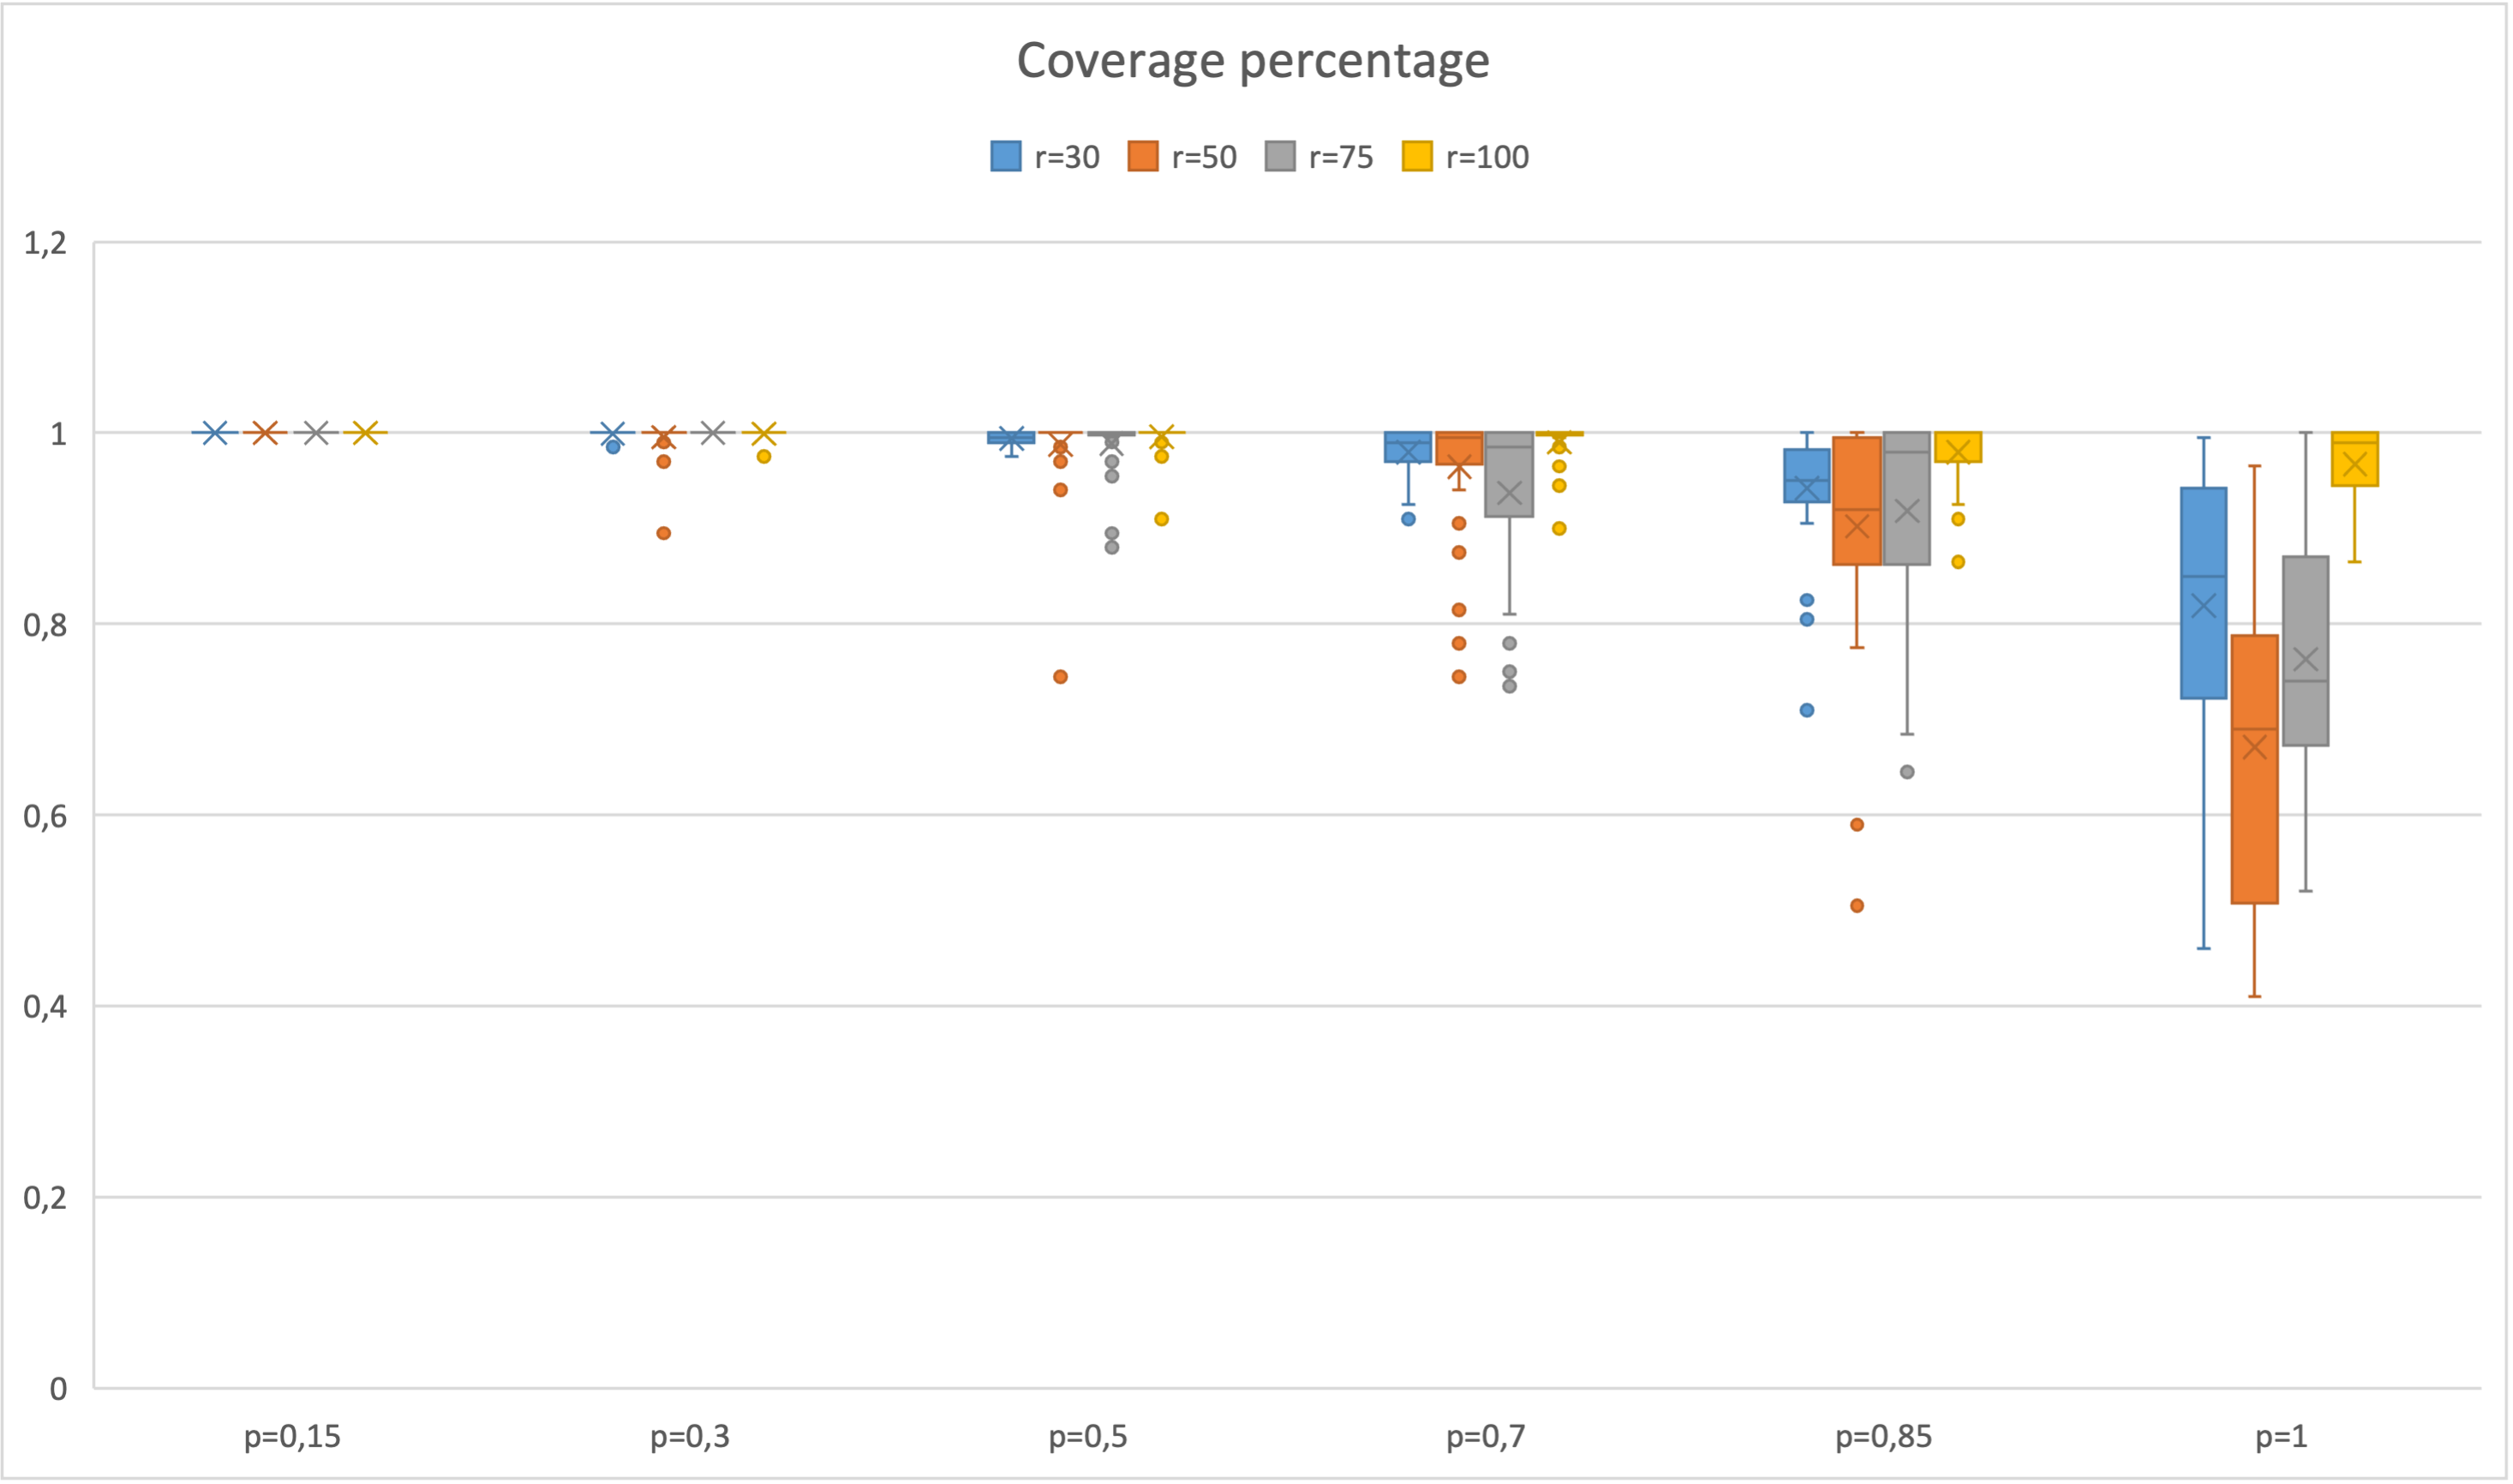
\includegraphics[width=\linewidth]{./images/Rate200Boxplot.png}
  \caption{200 Nodes}\label{fig:awesome_image2}
\endminipage
\end{figure}
\begin{figure}[H]
\minipage{0.50\linewidth}
  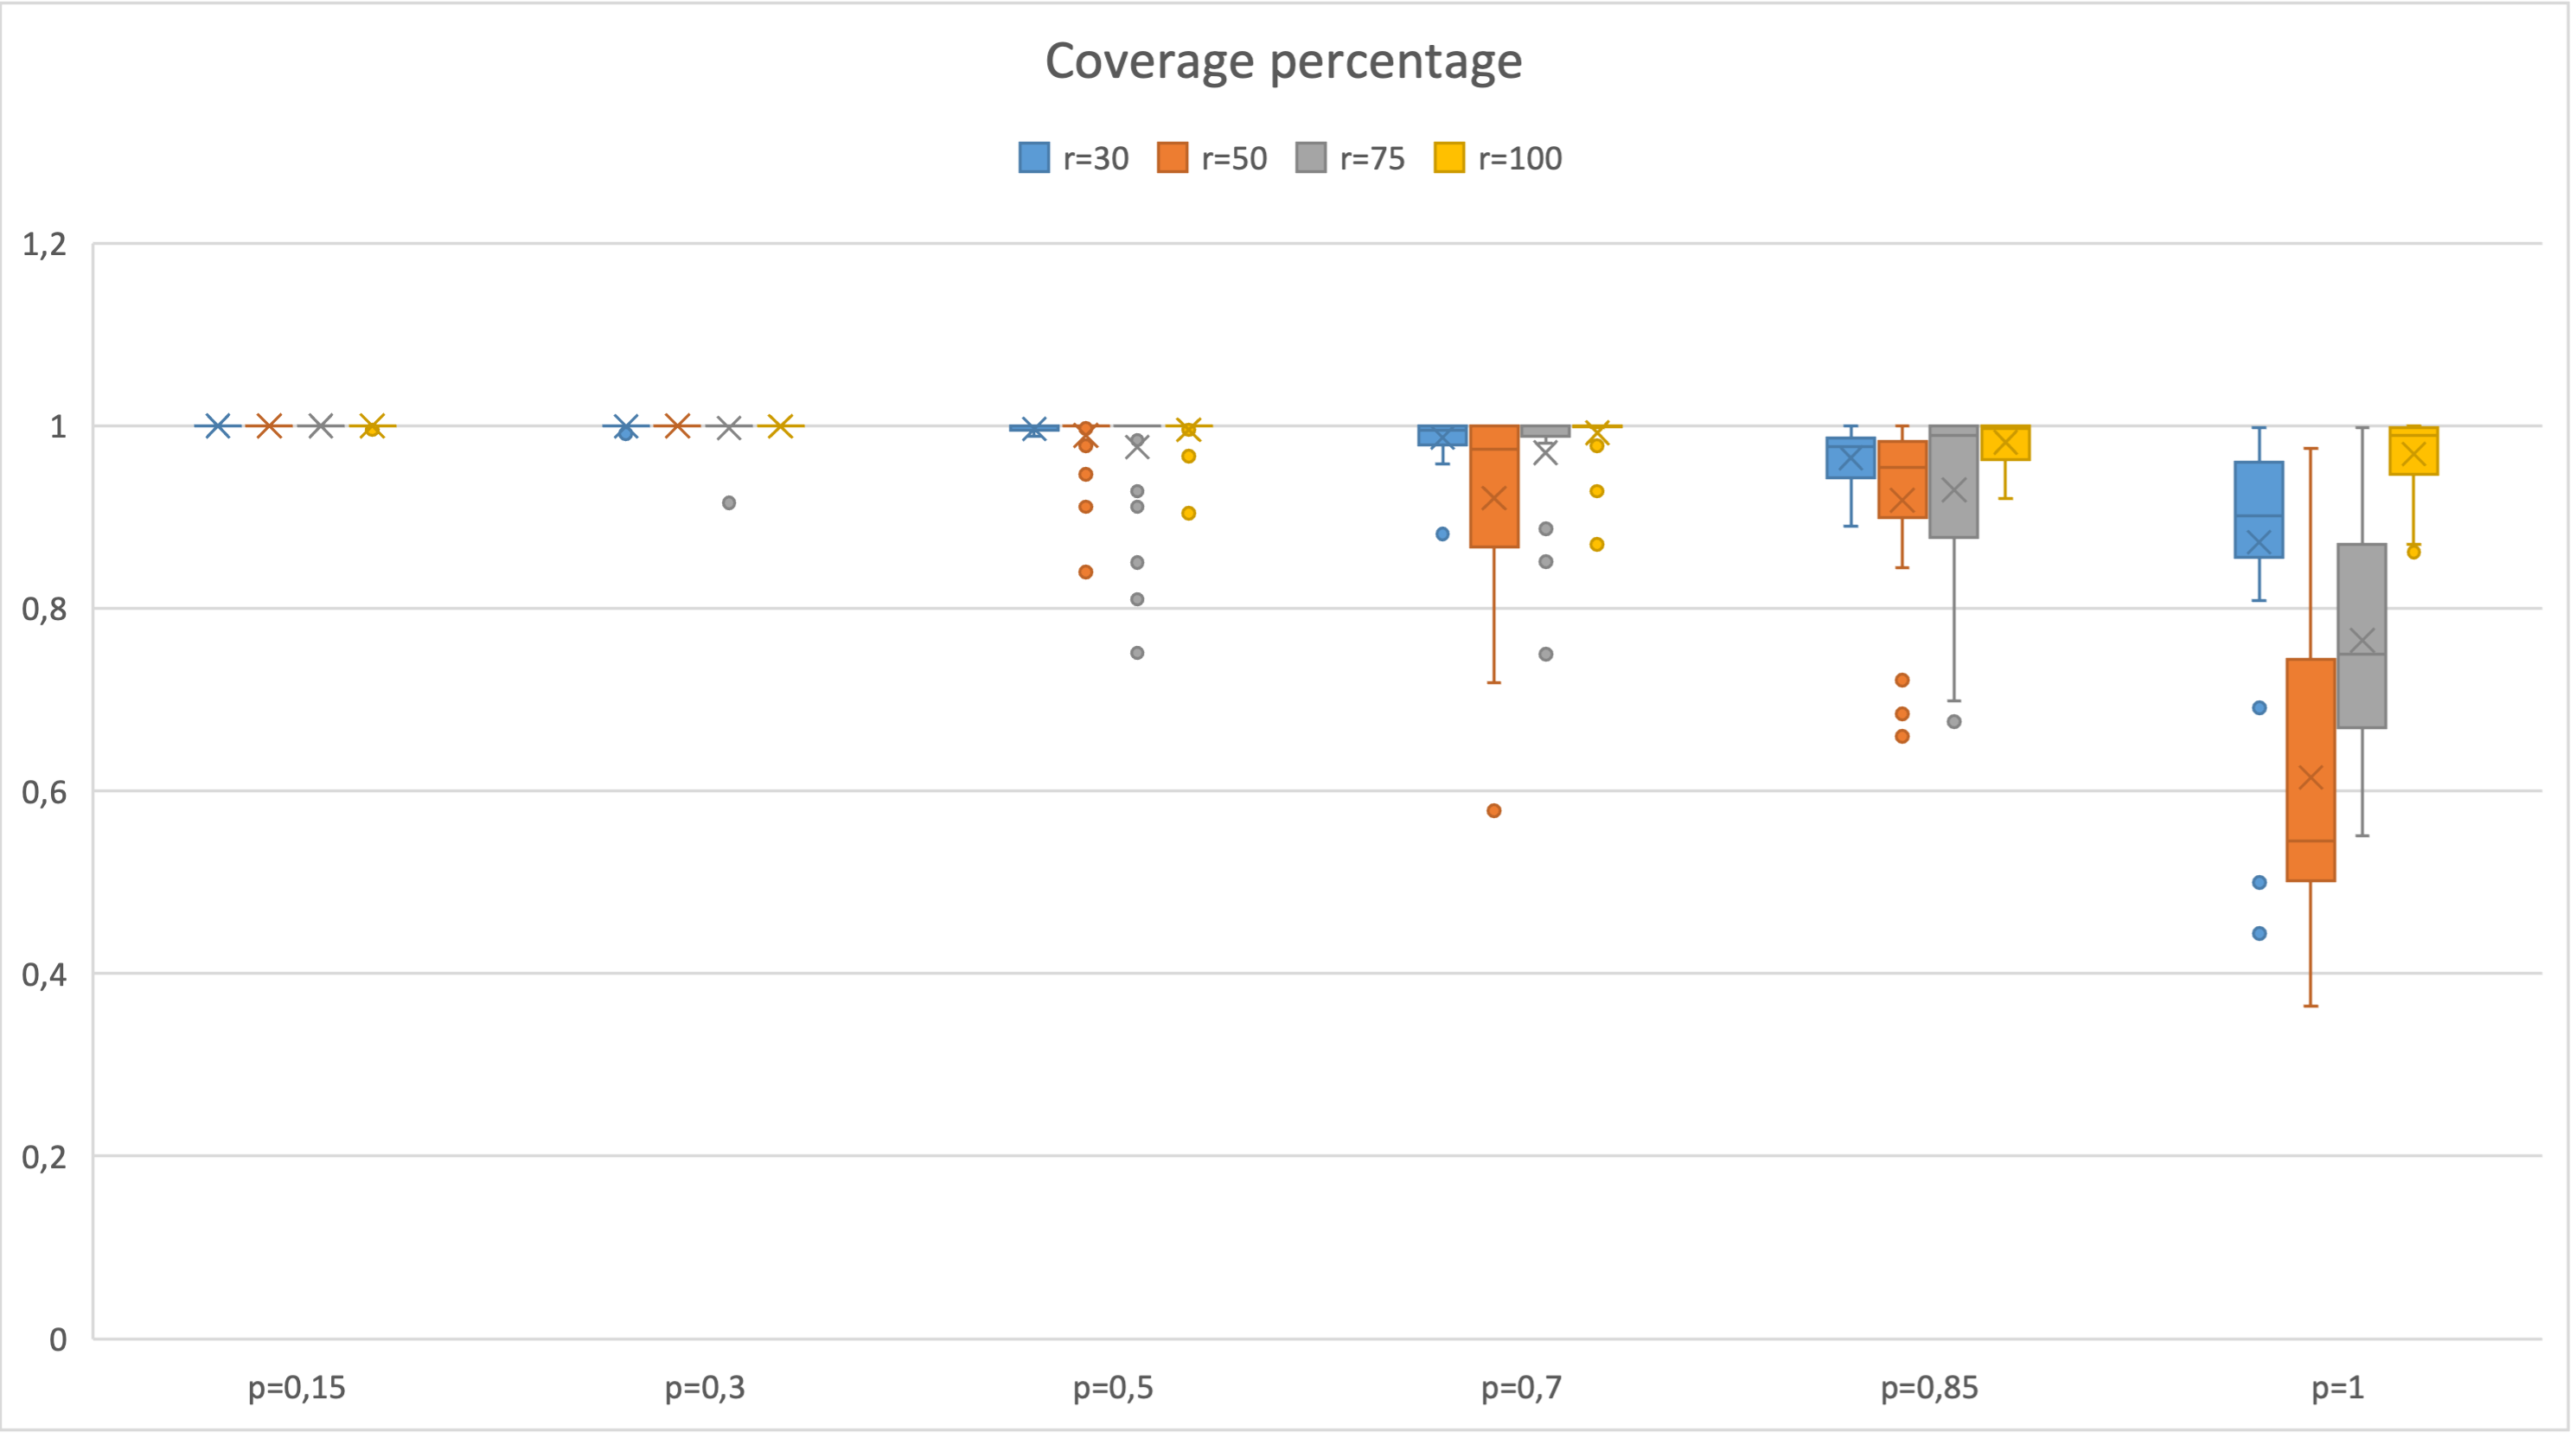
\includegraphics[width=\linewidth]{./images/Rate700Boxplot.png}
  \caption{700 Nodes}\label{fig:awesome_image1}
\endminipage\hfill
\minipage{0.50\linewidth}
  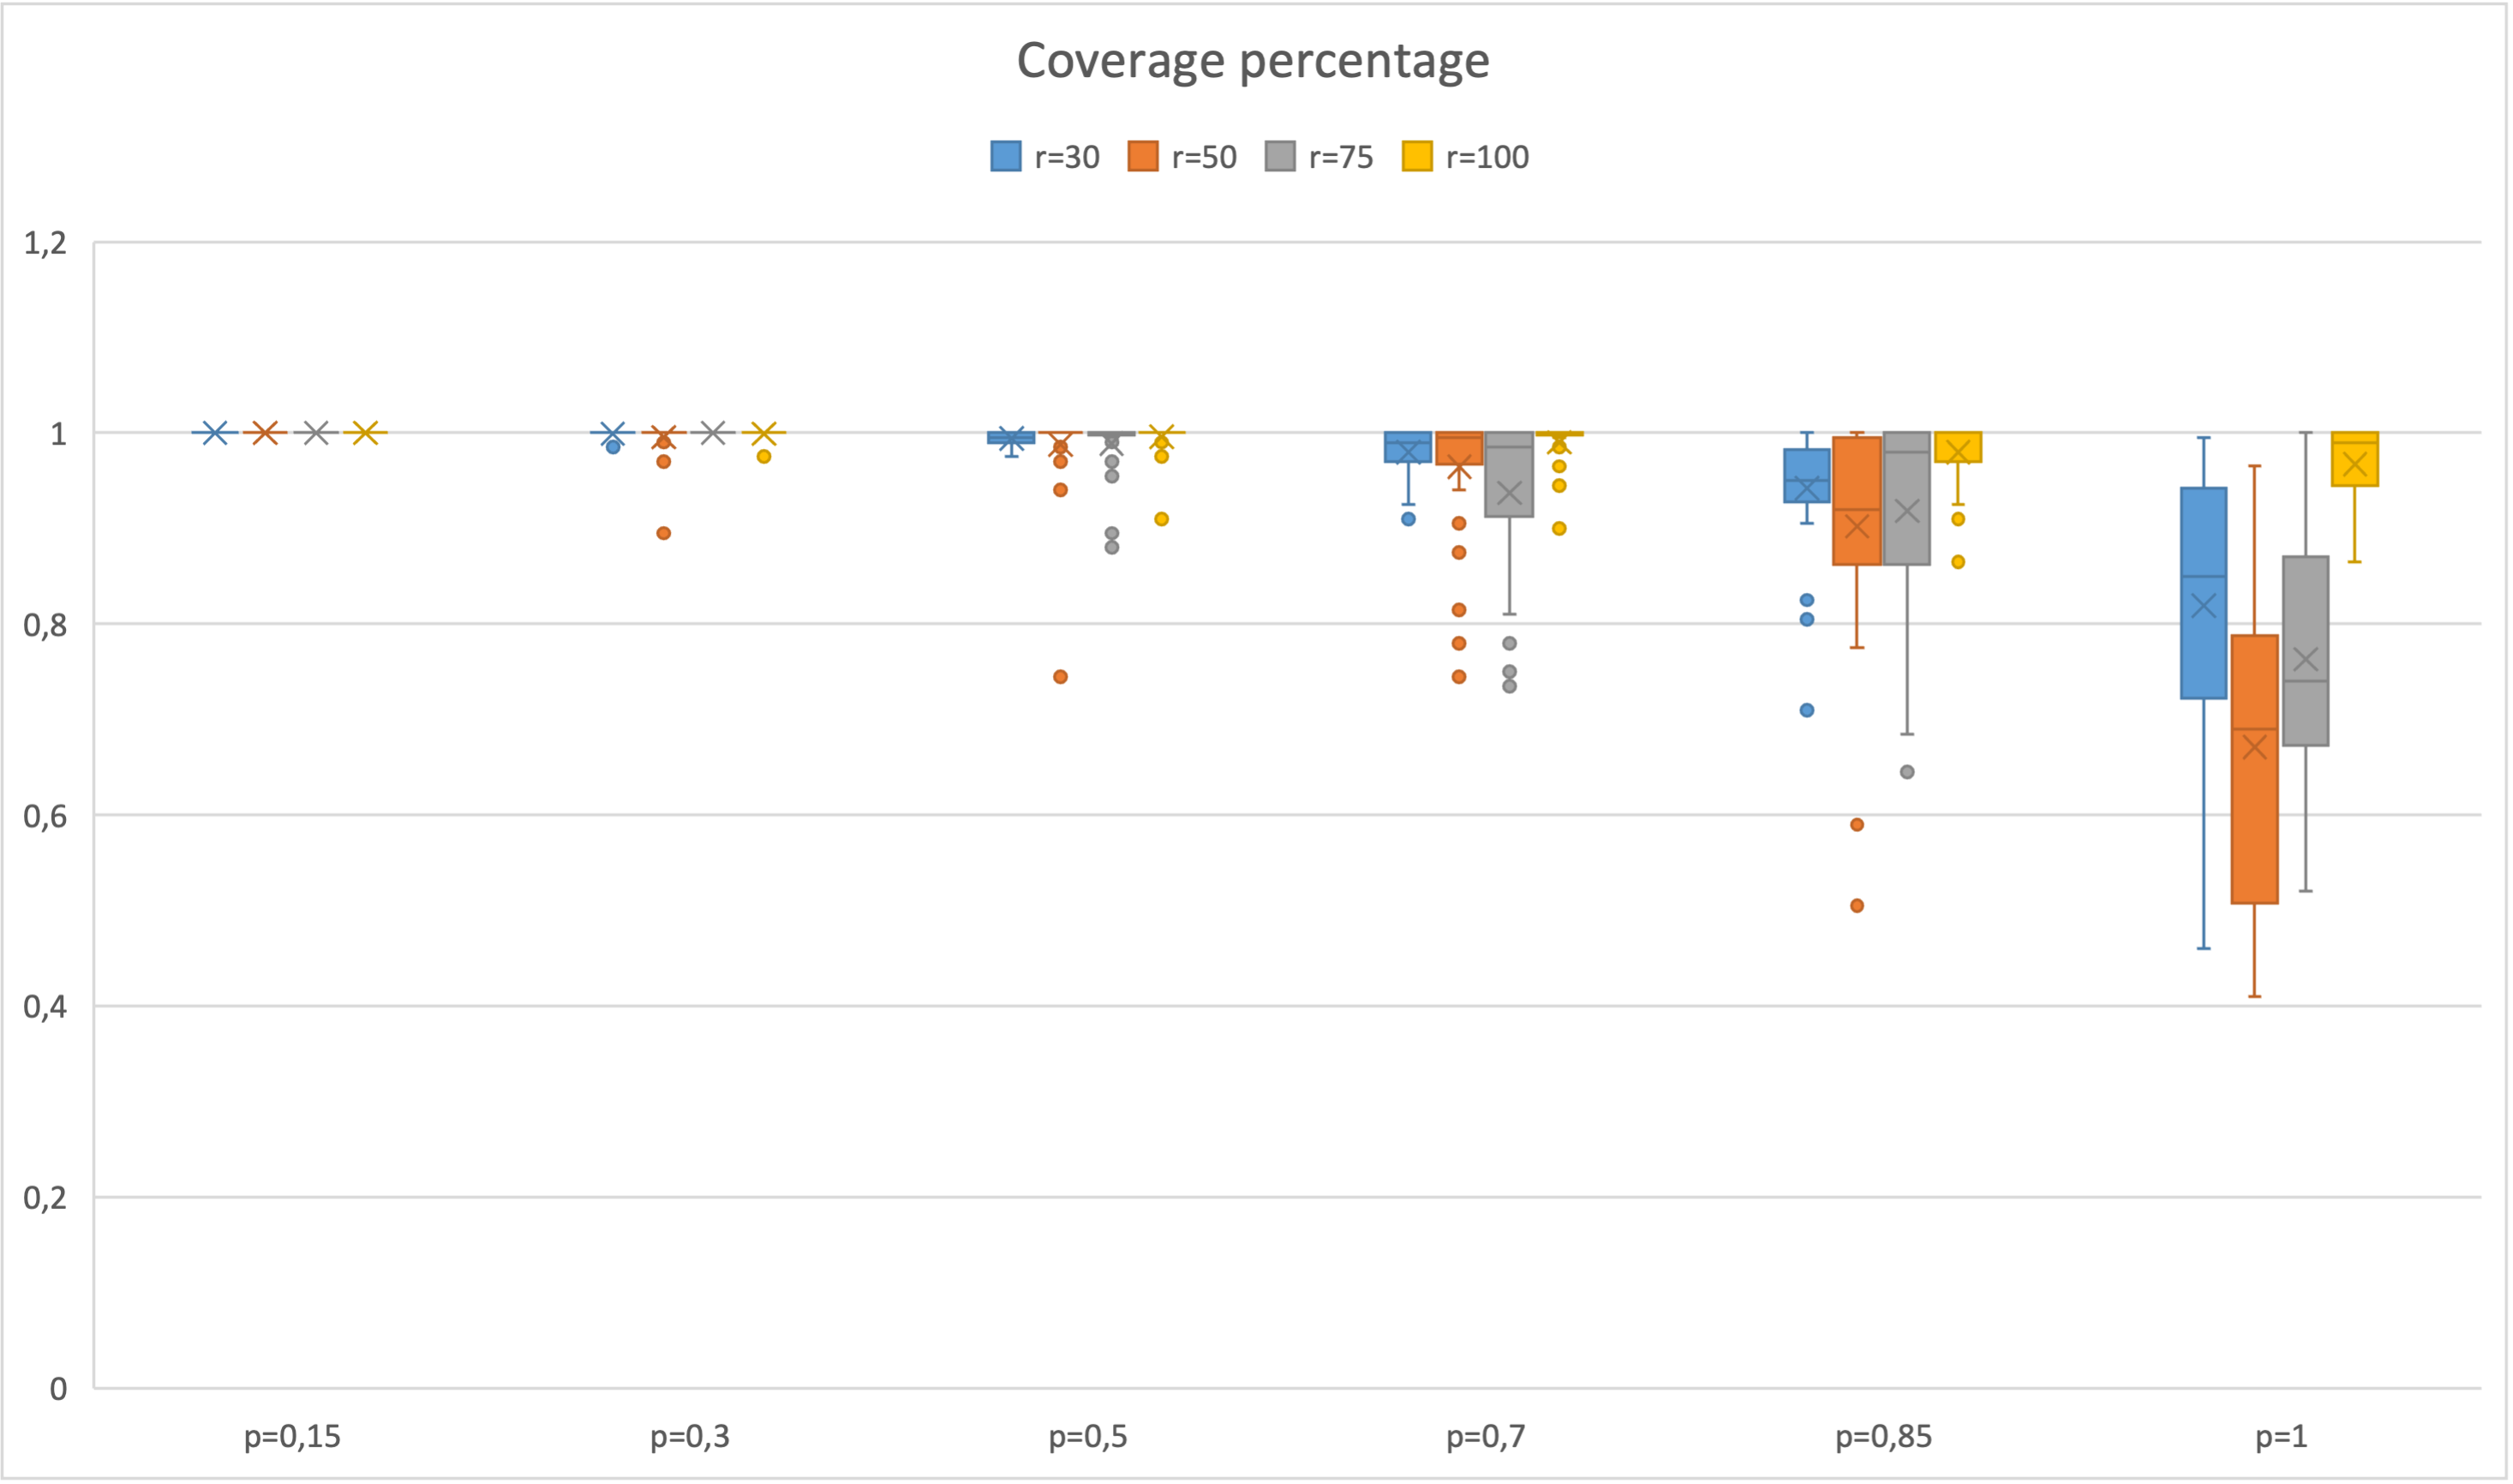
\includegraphics[width=\linewidth]{./images/Rate200Boxplot.png}
  \caption{200 Nodes}\label{fig:awesome_image2}
\endminipage
\end{figure}
